%- block legend
Given two integers $A$ and $B$, compute $A + B$.

Here is a diagram drawn with TikZ:

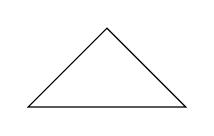
\begin{tikzpicture}
  \draw (0,0) -- (1,1) -- (2,0) -- cycle;
\end{tikzpicture}

A root-level static image: 
\includegraphics{pic}.

A nested static image: 
\includegraphics{img/diagram}.
%- endblock

%- block input
A single line with two integers $A$ and $B$.
%- endblock

%- block output
The sum $A + B$.
%- endblock

%- block notes
See the example explanation below.
%- endblock

%- block explanation_0
With $A = 3$ and $B = 7$, the answer is $10$.

The figure below illustrates the example:


\begin{tikzpicture}
  \draw (0,0) circle (0.5);
\end{tikzpicture}

And an attached image: 
\includegraphics{figs/expl}.
%- endblock
